% Los flotantes utilizan declaraciones de alineación y sus referencias e
% identificadores de imágenes contienen guiones intencionales.
% chktex-file 1
% chktex-file 8

\section{Qué se comprueba}

El análisis temporal comprueba que las rutas gobernadas por el reloj
puedan operar con el período de \SI{10}{\nano\second} definido para la
\tech{Basys 3} una vez ubicado y ruteado el circuito. A diferencia de
las simulaciones anteriores, esta etapa no evalúa resultados
aritméticos: analiza los retardos introducidos por los recursos y las
conexiones físicas elegidas por la herramienta.

\section{Resultado posterior al ruteo}

El resumen de timing presentó márgenes positivos de setup, hold y
ancho de pulso, sin endpoints fallidos. Los valores se reúnen en la
tabla~\ref{tab:timing} y se observan en la figura~\ref{fig:timing}.

\begin{table}[H]
	\centering
	\begin{tabularx}{\textwidth}{Y C{3.1cm} C{3.1cm} C{3.4cm}}
		\toprule
		\textbf{Análisis} & \textbf{Peor margen} & \textbf{Violación total}
		& \textbf{Endpoints con falla} \\
		\midrule
		Setup, WNS / TNS & \SI{7,224}{\nano\second} & \SI{0,000}{\nano\second} & 0 \\
		Hold, WHS / THS & \SI{0,128}{\nano\second} & \SI{0,000}{\nano\second} & 0 \\
		Ancho de pulso, WPWS / TPWS & \SI{4,500}{\nano\second} &
		\SI{0,000}{\nano\second} & 0 \\
		\bottomrule
	\end{tabularx}
	\caption{Resumen temporal posterior al ruteo.}%
	\label{tab:timing}
\end{table}

\begin{figure}[H]
	\centering
	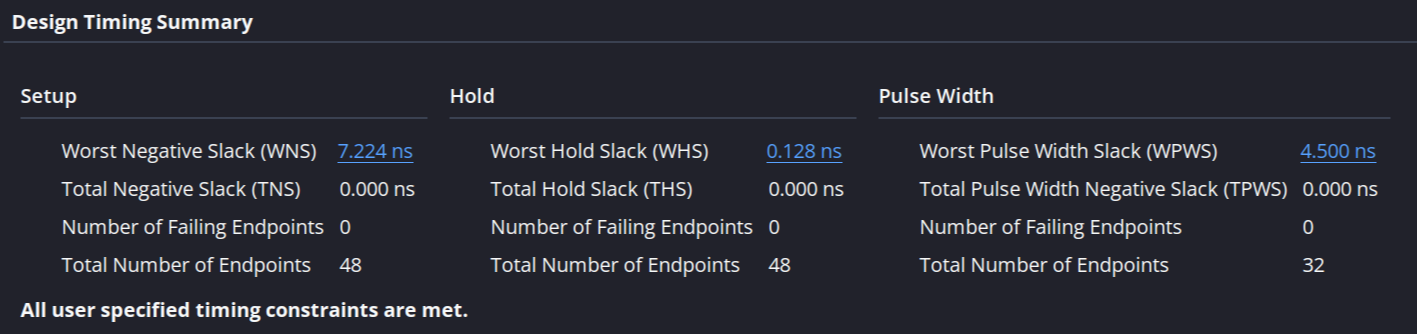
\includegraphics[width=\textwidth]{img/timing_summary.png}
	\caption{Cumplimiento de las restricciones temporales especificadas.}%
	\label{fig:timing}
\end{figure}

El WNS de \SI{7,224}{\nano\second} indica que la ruta de setup más
exigente conserva ese margen antes del límite de captura. El WHS de
\SI{0,128}{\nano\second} confirma que los datos también permanecen
estables durante el intervalo mínimo posterior al flanco. El análisis
consideró 48 endpoints para setup y hold y 32 para ancho de pulso,
todos sin violaciones.

El resultado permite afirmar que las rutas internas incluidas por las
restricciones cumplen el reloj de \SI{100}{\mega\hertz}.

\section{Validación sobre la placa}

Finalmente, la validación física se realizó sobre la \tech{Basys
3}. El bitstream se programó correctamente y el diseño funcionó en el
primer intento: no fue necesario modificar el RTL, las restricciones
ni la secuencia de carga. Los switches permitieron ingresar A, B y el
opcode mediante sus pulsadores correspondientes, y los LEDs mostraron
en todos los casos el resultado y los indicadores previstos.

Para conservar la relación entre cada fotografía y sus estímulos, los
archivos se nombraron como \texttt{OPERACION\_A\_B.jpeg}, con los
operandos expresados en hexadecimal. La
tabla~\ref{tab:physical-results} reúne los trece casos observados.
Las columnas Z, C y V corresponden, respectivamente, a cero, carry y overflow.

\begin{table}[H]
	\centering
	\small
	\begin{tabular}{lcccccc}
		\toprule
		\textbf{Operación} & \textbf{A} & \textbf{B} & \textbf{Resultado} &
		\textbf{Z} & \textbf{C} & \textbf{V} \\
		\midrule
		ADD & \texttt{80} & \texttt{80} & \texttt{00} & 1 & 1 & 1 \\
		ADD & \texttt{05} & \texttt{03} & \texttt{08} & 0 & 0 & 0 \\
		ADD & \texttt{7F} & \texttt{01} & \texttt{80} & 0 & 0 & 1 \\
		ADD & \texttt{FF} & \texttt{01} & \texttt{00} & 1 & 1 & 0 \\
		SUB & \texttt{05} & \texttt{05} & \texttt{00} & 1 & 0 & 0 \\
		SUB & \texttt{7F} & \texttt{FF} & \texttt{80} & 0 & 0 & 1 \\
		SUB & \texttt{80} & \texttt{01} & \texttt{7F} & 0 & 0 & 1 \\
		AND & \texttt{0C} & \texttt{0A} & \texttt{08} & 0 & 0 & 0 \\
		OR  & \texttt{A0} & \texttt{0F} & \texttt{AF} & 0 & 0 & 0 \\
		XOR & \texttt{AA} & \texttt{FF} & \texttt{55} & 0 & 0 & 0 \\
		NOR & \texttt{F0} & \texttt{0F} & \texttt{00} & 1 & 0 & 0 \\
		SRL & \texttt{80} & \texttt{01} & \texttt{40} & 0 & 0 & 0 \\
		SRA & \texttt{80} & \texttt{01} & \texttt{C0} & 0 & 0 & 0 \\
		\bottomrule
	\end{tabular}
	\caption{Resultados observados durante la validación física.}%
	\label{tab:physical-results}
\end{table}

Las fotografías siguientes muestran los LEDs después de completar cada
secuencia de carga. Las sumas y restas se reúnen en las
figuras~\ref{fig:physical-add} y~\ref{fig:physical-sub},
respectivamente. Las operaciones lógicas aparecen en la
figura~\ref{fig:physical-logic}, mientras que la
figura~\ref{fig:physical-shifts} permite comparar ambos desplazamientos.

\newcommand{\physicalcase}[2]{%
	\begin{minipage}[t]{0.47\textwidth}
		\centering
		\includegraphics[angle=90,width=\linewidth]{#1}\\[-0.15em]
		\small\texttt{#2}
	\end{minipage}%
}

\begin{figure}[H]
	\centering
	\physicalcase{img/ADD_80_80.jpeg}{ADD 80 80}\hfill
	\physicalcase{img/ADD_05_03.jpeg}{ADD 05 03}

	\par\vspace{0.8em}
	\physicalcase{img/ADD_7F_01.jpeg}{ADD 7F 01}\hfill
	\physicalcase{img/ADD_FF_01.jpeg}{ADD FF 01}
	\caption{Casos físicos de suma, incluidos cero, carry y overflow.}%
	\label{fig:physical-add}
\end{figure}

\clearpage
\begin{figure}[H]
	\centering
	\physicalcase{img/SUB_05_05.jpeg}{SUB 05 05}\hfill
	\physicalcase{img/SUB_7F_FF.jpeg}{SUB 7F FF}

	\par\vspace{0.8em}
	\physicalcase{img/SUB_80_01.jpeg}{SUB 80 01}
	\caption{Casos físicos de resta con resultado cero y overflow.}%
	\label{fig:physical-sub}
\end{figure}

\clearpage
\begin{figure}[H]
	\centering
	\physicalcase{img/AND_0C_0A.jpeg}{AND 0C 0A}\hfill
	\physicalcase{img/OR_A0_0F.jpeg}{OR A0 0F}

	\par\vspace{0.8em}
	\physicalcase{img/XOR_AA_FF.jpeg}{XOR AA FF}\hfill
	\physicalcase{img/NOR_F0_0F.jpeg}{NOR F0 0F}
	\caption{Validación física de las cuatro operaciones lógicas.}%
	\label{fig:physical-logic}
\end{figure}

\clearpage
\begin{figure}[H]
	\centering
	\physicalcase{img/SRL_80_01.jpeg}{SRL 80 01}\hfill
	\physicalcase{img/SRA_80_01.jpeg}{SRA 80 01}
	\caption{Diferencia observada entre los desplazamientos lógico y aritmético.}%
	\label{fig:physical-shifts}
\end{figure}

En los trece ensayos, el patrón de los LEDs coincidió con la salida
calculada y con los indicadores previstos en simulación. En
particular, el caso \texttt{80 + 80} produce \texttt{00} y activa
simultáneamente Z, C y V. Las fotografías también permiten observar
la diferencia entre carry y overflow, así como entre los modos de
desplazamiento lógico (SRL) y aritmético (SRA). Además, la carga
secuencial mediante pulsadores se comportó de manera estable durante
la prueba y no se observaron fallas que exigieran repetir la implementación.
